% D.24 切线长定理：P 外，PA、PB 切⊙O 于 A、B，∠APB=60°，OP=6
\documentclass[tikz,border=4pt]{standalone}
\usepackage{ctex}
\usepackage{amsmath}
\usetikzlibrary{calc}
\begin{document}
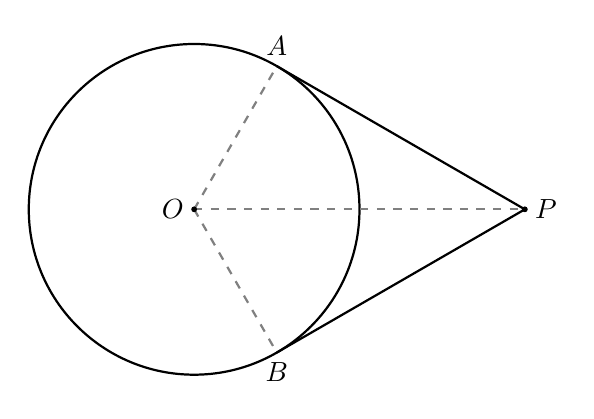
\begin{tikzpicture}[scale=0.7, thick]
  \coordinate (O) at (0, 0);
  \coordinate (P) at (6, 0);
  % ∠APB=60° → ∠APO=30° → OA = OP·sin(30°)=3
  \pgfmathsetmacro{\r}{3}
  \draw (O) circle (\r);
  % 切点 A、B：OA⊥PA，A 在直线 PA 上
  % 角 ∠OPA = 30°；A 位置：从 P 出发沿 (cos150°, sin150°) 方向（指向左上）距离 PA
  % PA = sqrt(OP^2-r^2)=sqrt(36-9)=sqrt(27)
  \pgfmathsetmacro{\pa}{sqrt(27)}
  \coordinate (A) at ({6 + \pa*cos(180-30)}, {\pa*sin(180-30)});
  \coordinate (B) at ({6 + \pa*cos(180+30)}, {\pa*sin(180+30)});

  \draw (P) -- (A);
  \draw (P) -- (B);
  \draw[gray, dashed] (O) -- (A);
  \draw[gray, dashed] (O) -- (B);
  \draw[gray, dashed] (O) -- (P);

  \fill (O) circle (1.5pt);
  \fill (P) circle (1.5pt);
  \node[left]  at (O) {$O$};
  \node[right] at (P) {$P$};
  \node[above] at (A) {$A$};
  \node[below] at (B) {$B$};
\end{tikzpicture}
\end{document}
